% !TEX program = xelatex
% !BIB program = bibtex

\documentclass[11pt,a4paper]{article}
\usepackage[UTF8]{ctex}
\usepackage{float}
\usepackage{amsmath}
\usepackage{amsfonts}
\usepackage{enumerate}
\usepackage{booktabs}
\usepackage{graphicx}
\usepackage{longtable}
\usepackage{subfigure}
\usepackage{multirow}
\usepackage{url}

% for reference 
\usepackage{hyperref}
\usepackage{cleveref}
\crefname{equation}{方程}{方程}
\Crefname{equation}{方程}{方程}
\crefname{table}{表}{表}
\Crefname{table}{表}{表}
\crefname{figure}{图}{图}
\Crefname{figure}{图}{图}

% Microsoft Word A4 paper default layout 
\usepackage[a4paper, left=3.18cm, right=3.18cm, top=2.54cm, bottom=2.54cm]{geometry}

\title{媒体计算实验二\\基于Seam Carving的图像智能缩放}
\author{2017011620 \quad 计73 \quad 李家昊}
\date{\today}

\begin{document}

\maketitle

\section{图像缩小}

我们首先考虑水平缩小的情形,根据基本的Seam Carving算法\cite{avidan2007seam},可以通过依次删除$n$条“最不重要”的8-连通竖直细缝,将图像的宽度减小$n$个像素,这样既保证了图像缩放自然,又保留了图像中的“重要内容”。

给定一张图像$I$,为了找出一条“最不重要”的竖直细缝,首先定义每个像素$(i,j)$的“重要性”为其能量值$E(i,j)$,像素的能量值可以通过多种方式来衡量,例如该点的梯度大小,即,
\begin{equation}
    E(i,j) = \left|\frac{\partial}{\partial x} I(i,j)\right| + \left|\frac{\partial}{\partial y} I(i,j)\right|
\end{equation}

像素的梯度越大,表明其越处于物体的边界位置,其重要性就越大。在具体实现中,$x,y$两个方向上的梯度可以通过Sobel算子对图像进行卷积计算得到,记Sobel卷积核为,
\begin{equation}
    G_x = \left(
    \begin{matrix}
        -1 & 0 & +1 \\
        -2 & 0 & +2 \\
        -1 & 0 & +1
    \end{matrix}
    \right),
    \quad
    G_y = \left(
    \begin{matrix}
        -1 & -2 & -1 \\
        0 & 0 & 0 \\
        +1 & +2 & +1
    \end{matrix}
    \right)
\end{equation}

则图像的能量可表示为,
\begin{equation}
    E(I) = |G_x * I| + |G_y * I|
\end{equation}

得到图像的能量后,可以通过动态规划,计算出从上往下到达每个位置$(i,j)$的细缝的累计最小能量$M(i,j)$,
\begin{equation}
    M(i,j) = E(i, j) + \min(M(i-1,j-1), M(i-1,j), M(i-1, j+1))
\end{equation}

其中边界条件为,
\begin{equation}
    M(0,j) = E(0, j)
\end{equation}

对矩阵$M$进行回溯,即可得到能量最小的细缝,即“最不重要”的细缝,将这一条细缝删除,即可将图像的宽度缩小1个像素。将上述过程迭代$n$次,即可将图像的宽度缩小$n$个像素,由于我们每次只删除了“最不重要”的细缝,图像的重要部分得以完好保留,同时保持自然。

对于竖直缩小的情形,考虑到上述过程的对称性,可以先将图像旋转$90^\circ$,进行水平缩小后,再逆向旋转$90^\circ$回到初始位置,这样就实现了竖直缩小。

水平缩小结果如\Cref{fig:narrow_x},可以看出天空部分被缩小,而人和城堡这些重要部分都被完整保留;竖直缩小结果如\Cref{fig:narrow_y},天空部分同样被缩小,而富士山和海浪都基本完好保存。

\begin{figure}[H]
    \centering
    \subfigure[原始图像]{
        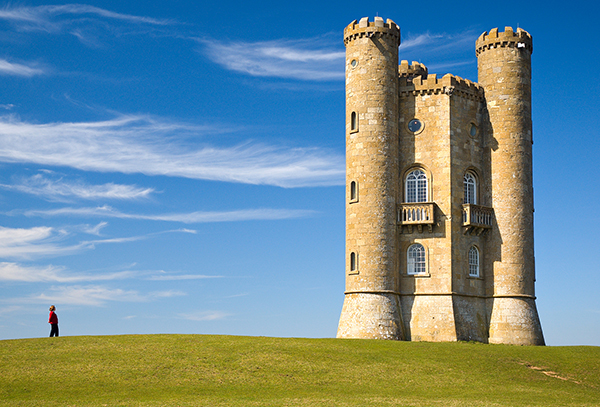
\includegraphics[height=4.0cm]{../src/fig/castle.jpg}
    }
    \subfigure[水平缩小]{
        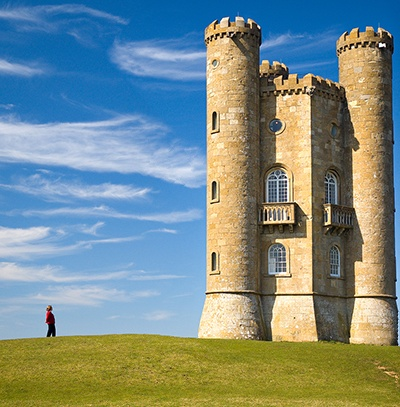
\includegraphics[height=4.0cm]{../src/output/castle_down.jpg}
    }
    \caption{水平缩小效果}
    \label{fig:narrow_x}
\end{figure}

\begin{figure}[H]
    \centering
    \subfigure[原始图像]{
        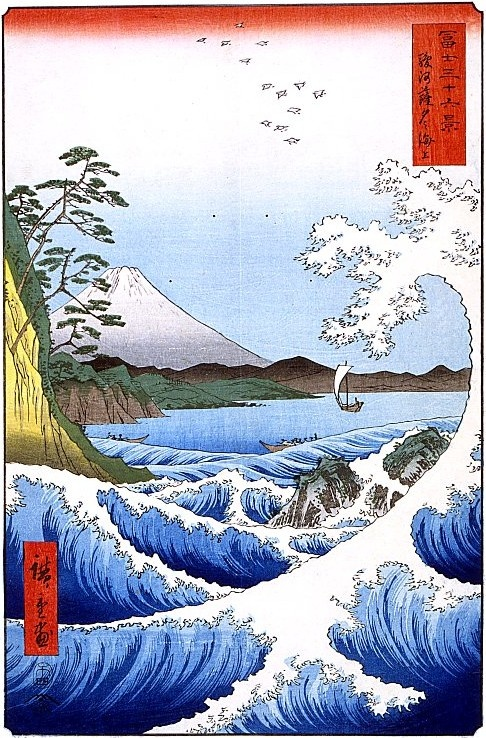
\includegraphics[width=3.5cm]{../src/fig/fuji.jpg}
    }
    \subfigure[竖直缩小]{
        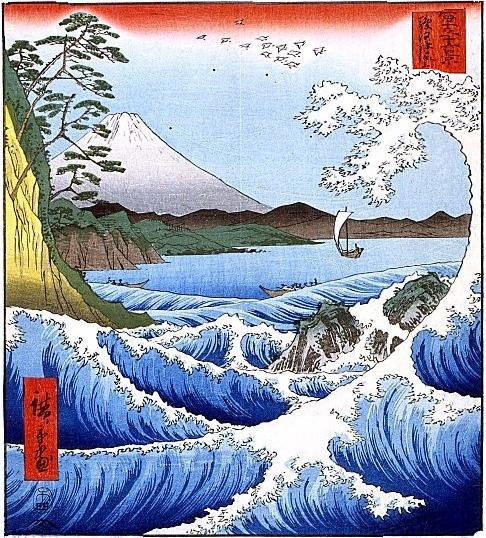
\includegraphics[width=3.5cm]{../src/output/fuji_down_y.jpg}
    }
    \caption{竖直缩小效果}
    \label{fig:narrow_y}
\end{figure}

然而,Seam Carving在某些情况下效果不佳,例如\Cref{fig:failure_case},这是因为图像的“重要内容”分布不均:右方的重要内容为城堡,因此算法删减草地,左方的重要内容是人和草地,因此删减天空,导致最终画面的不平衡。

\begin{figure}[H]
    \centering
    \subfigure[原始图像]{
        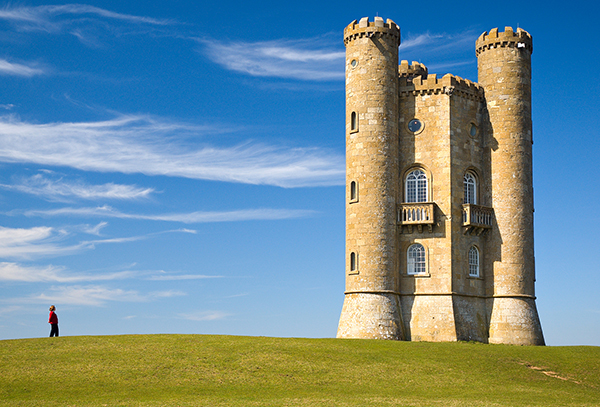
\includegraphics[width=5.0cm]{../src/fig/castle.jpg}
    }
    \subfigure[竖直缩小]{
        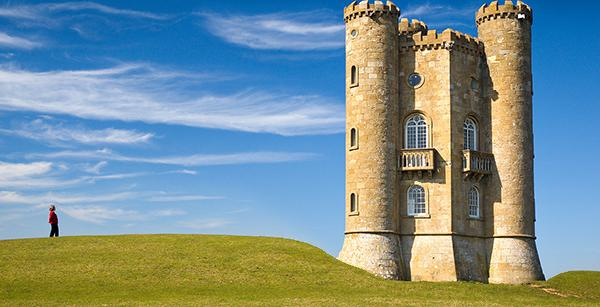
\includegraphics[width=5.0cm]{../src/output/castle_down_y.jpg}
    }
    \caption{一个失败的例子}
    \label{fig:failure_case}
\end{figure}

\section{多种能量函数}

图像的能量可用多种方式衡量,这里实现了$e_1$,$e_{Entropy}$和$e_{HoG}$三种能量函数。

对于$e_1$能量,我们求出$x,y$两个方向上的梯度的1范数,作为该像素的能量。
\begin{equation}
    e_1(x,y) = \left|\frac{\partial}{\partial x} I(i,j)\right| + \left|\frac{\partial}{\partial y} I(i,j)\right|
\end{equation}

对于$e_{Entropy}$能量,我们在$e_1$能量的基础上,加上以该像素为中心的$9\times 9$滑动窗口的图像熵。
\begin{equation}
    e_{Entropy}(x,y) = e_1(x,y) + Entropy(I(x, y))
\end{equation}

对于$e_{HoG}$能量,我们需要求出$11\times 11$滑动窗口的梯度直方图中的最大值,作为$e_1$能量的归一化因子。
\begin{equation}
    e_{HoG}(x,y) = \frac{e_1(x,y)}{\max(HoG(I(x,y)))}    
\end{equation}

我们将\Cref{fig:charles}作为原始图像,分别采用三种能量函数进行Seam Carving,结果如\Cref{fig:energy}。

\begin{figure}[H]
    \centering
    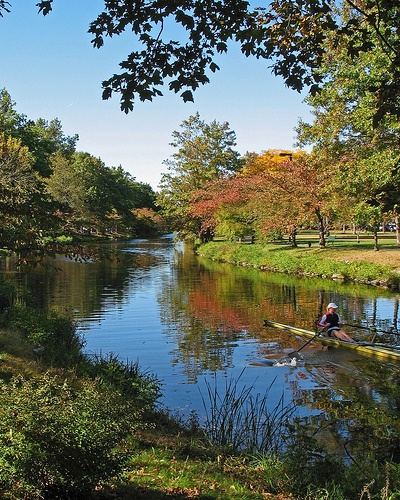
\includegraphics[width=0.5\textwidth]{../src/fig/charles.jpg}
    \caption{原始图像}
    \label{fig:charles}
\end{figure}

\begin{figure}[H]
    \centering
    \subfigure[$e_1$能量]{
        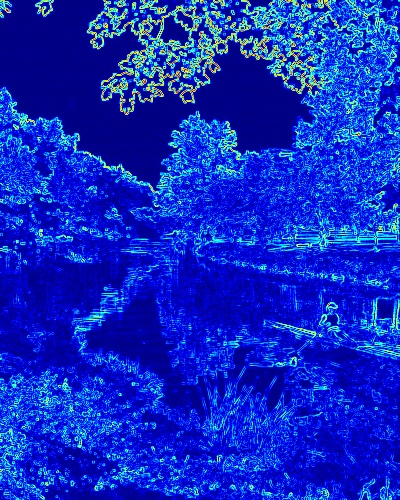
\includegraphics[width=0.3\textwidth]{../src/output/charles_e1_energy.jpg}
    }
    \subfigure[$e_1$累计能量]{
        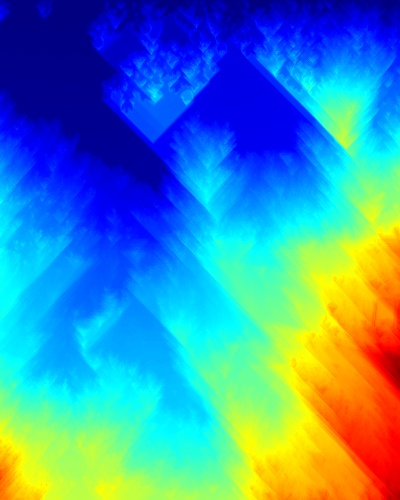
\includegraphics[width=0.3\textwidth]{../src/output/charles_e1_cost.jpg}
    }
    \subfigure[$e_1$能量缩小结果]{
        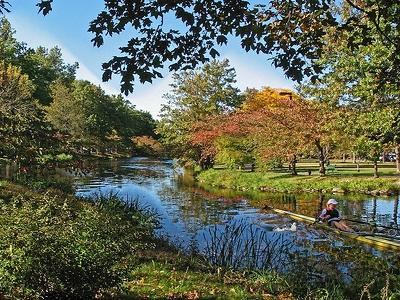
\includegraphics[width=0.3\textwidth]{../src/output/charles_e1_down.jpg}
    }
    \subfigure[$e_{Entropy}$能量]{
        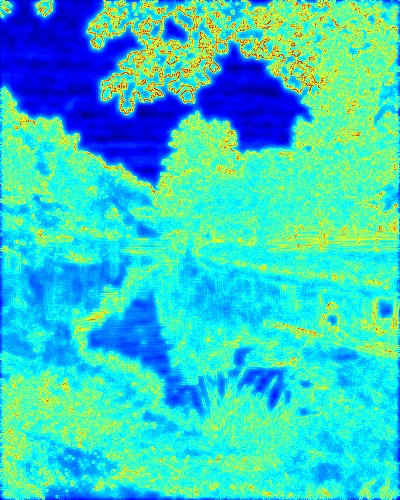
\includegraphics[width=0.3\textwidth]{../src/output/charles_entropy_energy.jpg}
    }
    \subfigure[$e_{Entropy}$累计能量]{
        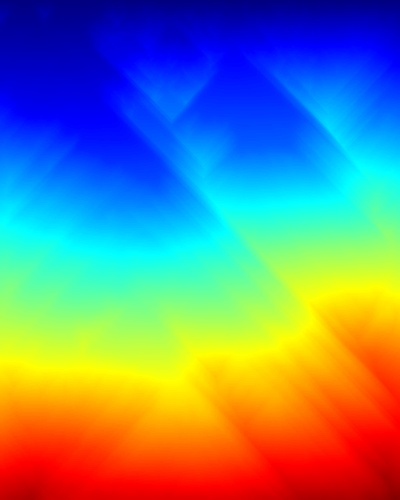
\includegraphics[width=0.3\textwidth]{../src/output/charles_entropy_cost.jpg}
    }
    \subfigure[$e_{Entropy}$能量缩小结果]{
        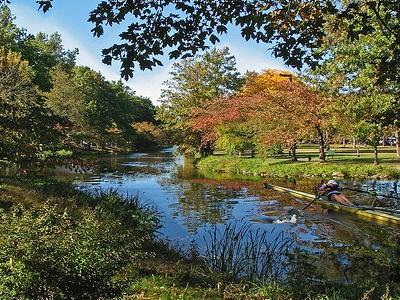
\includegraphics[width=0.3\textwidth]{../src/output/charles_entropy_down.jpg}
    }
    \subfigure[$e_{HoG}$能量]{
        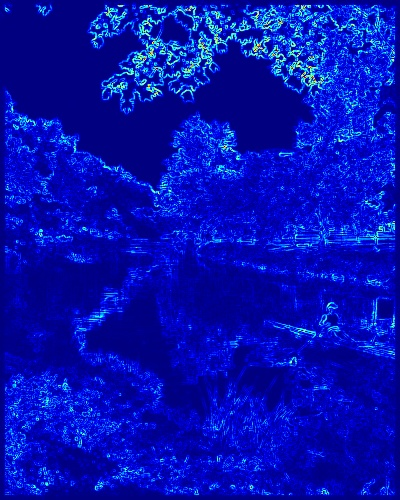
\includegraphics[width=0.3\textwidth]{../src/output/charles_hog_energy.jpg}
    }
    \subfigure[$e_{HoG}$累计能量]{
        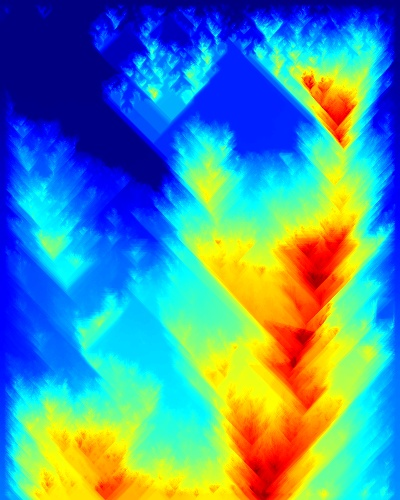
\includegraphics[width=0.3\textwidth]{../src/output/charles_hog_cost.jpg}
    }
    \subfigure[$e_{HoG}$能量缩小结果]{
        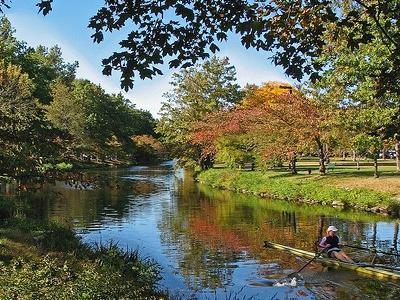
\includegraphics[width=0.3\textwidth]{../src/output/charles_hog_down.jpg}
    }
    \caption{多种能量函数效果对比}
    \label{fig:energy}
\end{figure}

\section{图像扩展}

\subsection{迭代扩展}

基于Seam Carving算法,我们同样可以实现图像扩展。在图像缩小的情形中,我们每次删除图像中能量最小的细缝;受此启发,如果我们每次在最小细缝中扩充一个像素,取值为细缝两旁像素的平均值,迭代$n$次就能将图像的宽度扩展$n$个像素,这样就实现了图像的迭代扩展,效果如\Cref{fig:iter_expand}。

\begin{figure}[H]
    \centering
    \subfigure[原图]{
        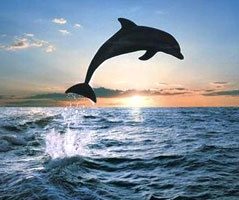
\includegraphics[height=4.5cm]{../src/fig/dolphin.jpg}
    }
    \subfigure[迭代扩展]{
        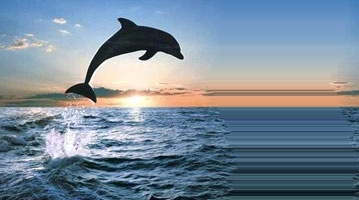
\includegraphics[height=4.5cm]{../src/output/dolphin_iter_expand.jpg}
    }
    \caption{迭代扩展效果}
    \label{fig:iter_expand}
\end{figure}

\subsection{统一扩展}

然而,上述迭代扩展的效果并不理想,原因是算法每次找到的最小细缝都可能是相同的,导致同一条细缝的像素被多次复制。为了解决这个问题,我们可以在原图上统一计算出能量最小的前$n$条细缝,统一扩展这$n$条细缝,从而避免重复扩展同一条细缝,效果如\Cref{fig:opt_expand}。

\begin{figure}[H]
    \centering
    \subfigure[原图]{
        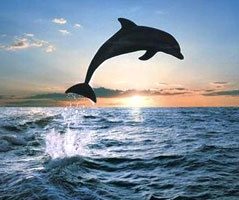
\includegraphics[height=4.5cm]{../src/fig/dolphin.jpg}
    }
    \subfigure[统一扩展]{
        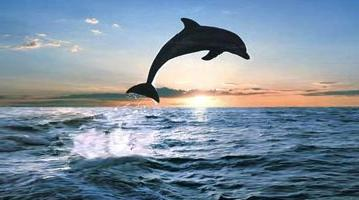
\includegraphics[height=4.5cm]{../src/output/dolphin_expand.jpg}
    }
    \caption{统一扩展效果}
    \label{fig:opt_expand}
\end{figure}

\subsection{分阶段扩展}

在统一扩展的情形中,图像每次扩展的宽度不能超过图像原本的宽度,在实际应用中,应当进一步限制每次扩展宽度的上限,保证扩展效果。如果图像需要扩展的宽度超出了上限,可以进行分阶段扩展,每个阶段在上一阶段的输出图像上继续扩展,直到满足扩展宽度要求,结果如\Cref{fig:seg_expand}。

\begin{figure}[H]
    \centering
    \subfigure[原图]{
        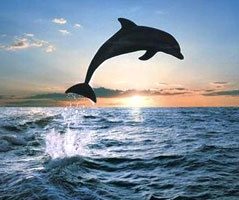
\includegraphics[height=3cm]{../src/fig/dolphin.jpg}
    }
    \subfigure[一阶段扩展]{
        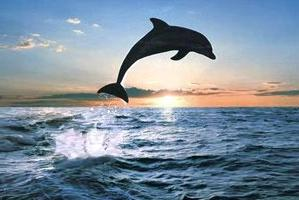
\includegraphics[height=3cm]{../src/output/dolphin_expand_1.jpg}
    }
    \subfigure[二阶段扩展]{
        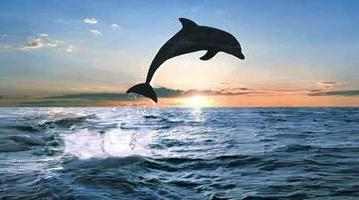
\includegraphics[height=3cm]{../src/output/dolphin_expand_2.jpg}
    }
    \caption{分阶段扩展效果}
    \label{fig:seg_expand}
\end{figure}

\section{目标保护和移除}

在基本的Seam Carving算法中,我们每次移除能量最小的一条细缝,因此我们可以通过重新加权图像的能量,引导整个细缝删除的过程,高效地保护或移除目标。

对于目标保护,我们把目标像素的能量统一提高一个常数$E_p$,使得细缝难以经过目标像素;对于目标移除,我们把目标像素的能量统一降低一个常数$E_r$,使得细缝优先经过目标像素。在具体实现中,我们必须采用移除优先策略,即保证$E_r \gg E_p$,否则在目标保护和目标移除并存的情形中,移除目标的代价将极其巨大。

目标移除的结果如\Cref{fig:remove_object},其中物体的分割可通过photoshop抠图得到,在去掉物体后,这里进一步采用Seam Carving的方法将图像扩展到原始大小。

目标保护的结果如\Cref{fig:protect_shoes},其中绿色掩膜表示需要保护的目标,红色掩膜表示需要移除的目标。

\begin{figure}[H]
    \centering
    \subfigure[原始图像]{
        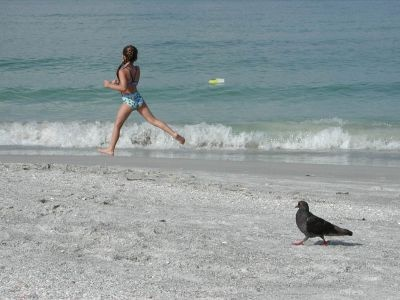
\includegraphics[height=2.5cm]{../src/fig/beach.jpg}
    }
    \subfigure[女孩的掩膜]{
        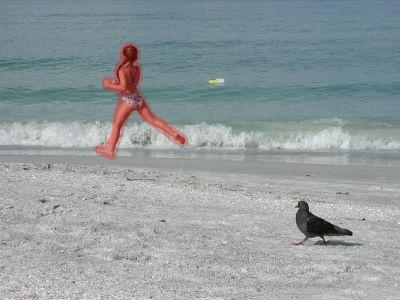
\includegraphics[height=2.5cm]{../src/output/beach_overlay.jpg}
    }
    \subfigure[去掉女孩]{
        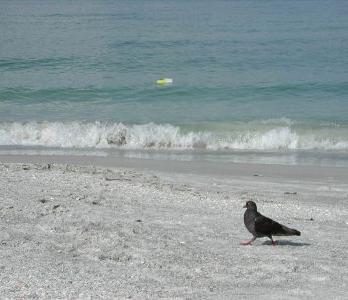
\includegraphics[height=2.5cm]{../src/output/beach_no_girl.jpg}
    }
    \subfigure[扩展到原始大小]{
        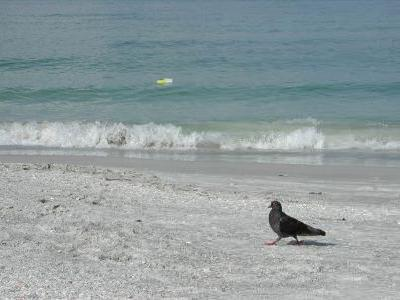
\includegraphics[height=2.5cm]{../src/output/beach_no_girl_resized.jpg}
    }
    \caption{移除目标}
    \label{fig:remove_object}
\end{figure}

\begin{figure}[H]
    \centering
    \subfigure[原始图像]{
        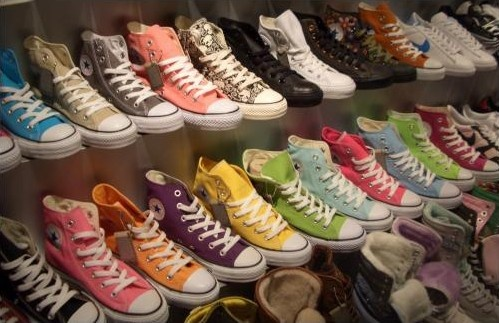
\includegraphics[height=2.2cm]{../src/fig/shoes.jpg}
    }
    \subfigure[鞋子的掩膜]{
        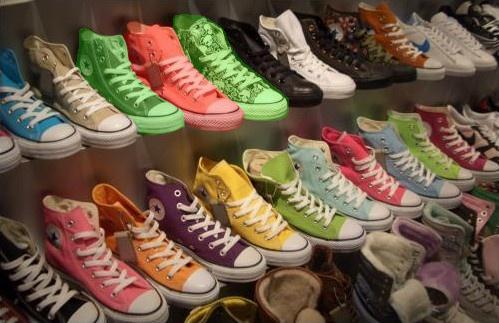
\includegraphics[height=2.2cm]{../src/output/shoes_overlay.jpg}
    }
    \subfigure[去掉鞋子]{
        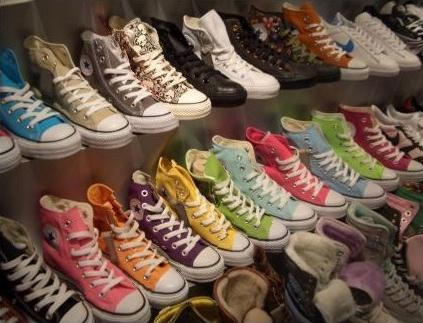
\includegraphics[height=2.2cm]{../src/output/shoes_removed.jpg}
    }
    \subfigure[扩展到原始大小]{
        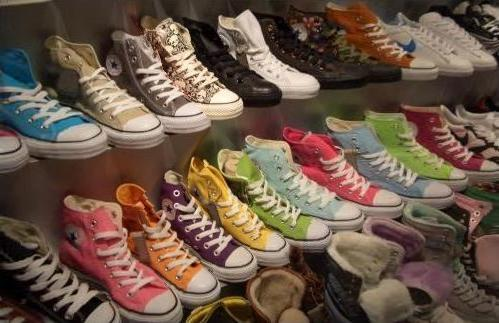
\includegraphics[height=2.2cm]{../src/output/shoes_removed_resized.jpg}
    }
    \caption{保护目标的同时移除另一个目标}
    \label{fig:protect_shoes}
\end{figure}

\section{改进能量公式}

\subsection{前向能量}

为了改善算法效果,研究者在改进的Seam Carving算法\cite{rubinstein2008improved}中提出了前向能量公式。在基本的Seam Carving算法中,我们考虑的是图像中每个像素自身的能量,即后向能量;而在前向能量中,我们考虑的是细缝删除后产生的相邻像素的能量,如\Cref{fig:forward_dp}。

\begin{figure}[H]
    \centering
    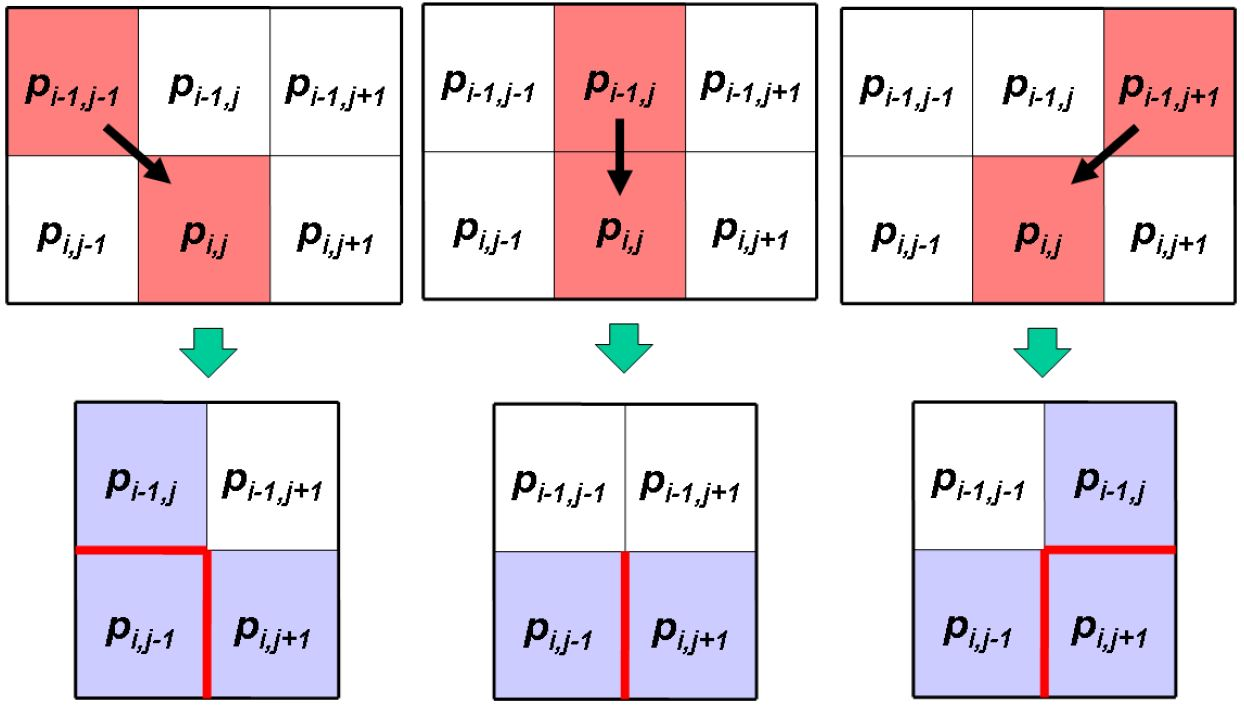
\includegraphics[width=0.6\textwidth]{../src/fig/forward_dp.jpg}
    \caption{前向能量原理}
    \label{fig:forward_dp}
\end{figure}

对于一个像素$(i,j)$,考虑细缝穿过上层像素的位置。如果细缝穿过像素的正上方,则细缝删除后像素$(i,j-1)$与$(i,j+1)$相邻,其能量记为$C_U$;如果细缝穿过像素的左上方,则像素$(i,j-1)$与$(i,j+1)$相邻,$(i-1,j)$与$(i,j-1)$相邻,能量记为$C_L$;如果细缝穿过像素的右上方,则像素$(i,j-1)$与$(i,j+1)$相邻,$(i-1,j)$与$(i,j+1)$相邻,能量记为$C_R$。即,
\begin{equation}
    \begin{split}
        C_L(i,j) &= |I(i,j+1)-I(i,j-1)| + |I(i-1,j)-I(i,j-1)|\\
        C_U(i,j) &= |I(i,j+1)-I(i,j-1)|\\
        C_R(i,j) &= |I(i,j+1)-I(i,j-1)| + |I(i-1,j)-I(i,j+1)|
    \end{split}
\end{equation}

对上述能量进行动态规划,即可求出到达每个位置$(i,j)$的累计最小能量$M(i,j)$,
\begin{equation}
    M(i,j) = \begin{cases}
        M(i-1,j-1) + C_L(i,j)\\
        M(i-1,j) + C_U(i,j)\\
        M(i-1,j+1) + C_R(i,j)
    \end{cases}
\end{equation}

与后向能量类似,可以通过回溯求出能量最小的细缝,最终结果如\Cref{fig:forward_energy}。

\begin{figure}[H]
    \centering
    \subfigure[后向能量]{
        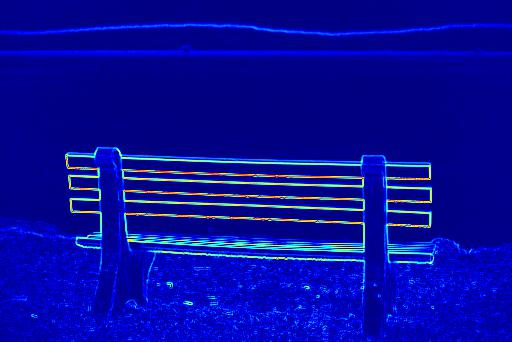
\includegraphics[height=2.3cm]{../src/output/bench_backward_energy.jpg}
    }
    \subfigure[后向累计能量]{
        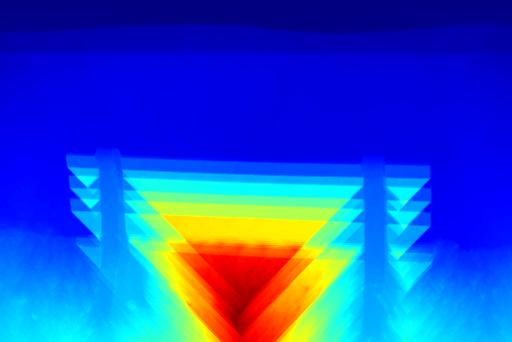
\includegraphics[height=2.3cm]{../src/output/bench_backward_cost.jpg}
    }
    \subfigure[后向能量细缝]{
        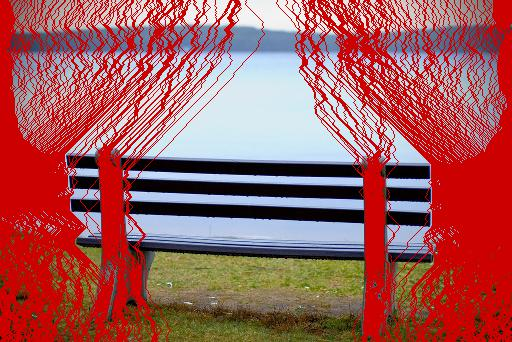
\includegraphics[height=2.3cm]{../src/output/bench_backward_seams.jpg}
    }
    \subfigure[后向结果]{
        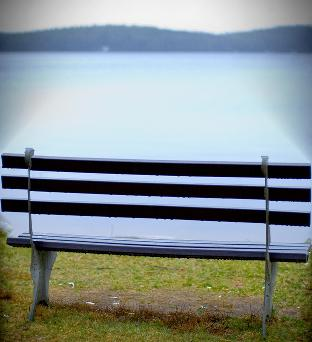
\includegraphics[height=2.3cm]{../src/output/bench_backward.jpg}
    }
    \subfigure[前向能量]{
        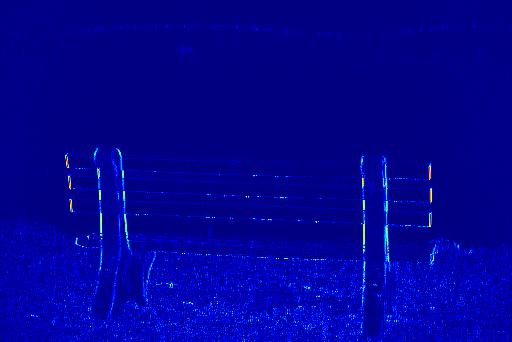
\includegraphics[height=2.3cm]{../src/output/bench_forward_energy.jpg}
    }
    \subfigure[前向累计能量]{
        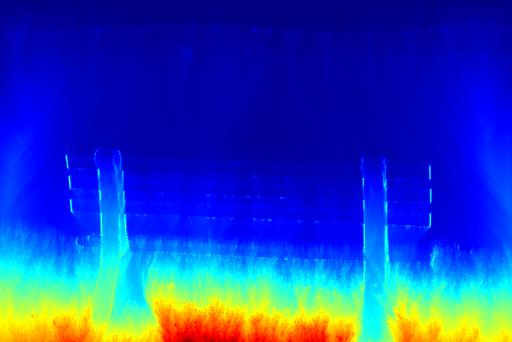
\includegraphics[height=2.3cm]{../src/output/bench_forward_cost.jpg}
    }
    \subfigure[前向能量细缝]{
        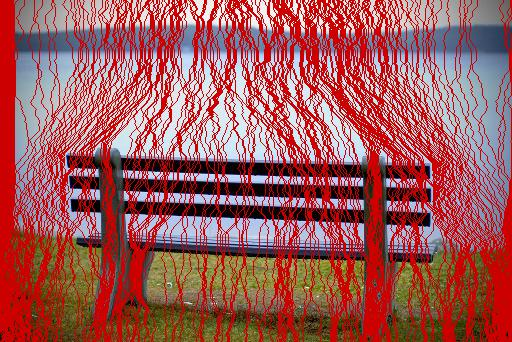
\includegraphics[height=2.3cm]{../src/output/bench_forward_seams.jpg}
    }
    \subfigure[前向结果]{
        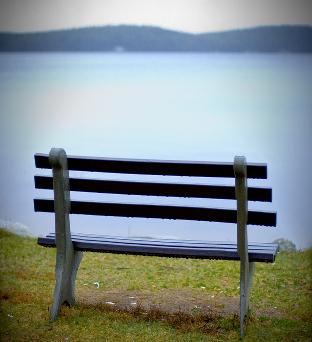
\includegraphics[height=2.3cm]{../src/output/bench_forward.jpg}
    }
    \caption{前向能量与后向能量}
    \label{fig:forward_energy}
\end{figure}

\subsection{处理人脸}

人脸具有很强的结构化信息,人眼对它十分敏感,如果图像中存在人脸,算法可能会裁剪人脸中不合适的部分,导致输出的人脸非常扭曲,如\Cref{fig:face_unprotect}。

\begin{figure}[H]
    \centering
    \subfigure[原始图像]{
        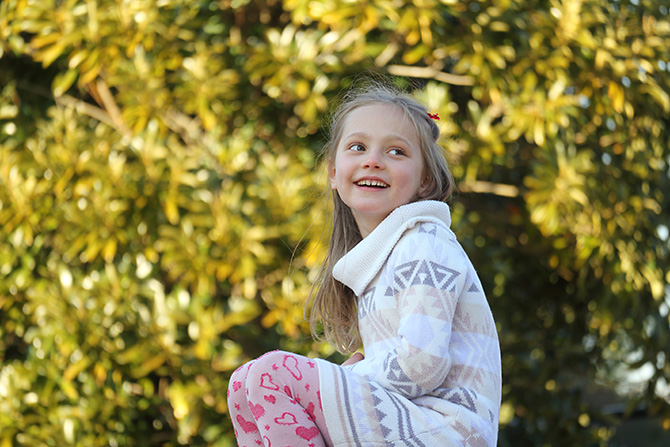
\includegraphics[height=4.0cm]{../src/fig/face.jpg}
    }
    \subfigure[图像缩小]{
        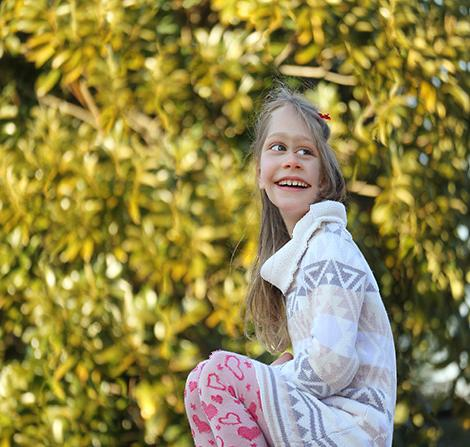
\includegraphics[height=4.0cm]{../src/output/face_unprotect.jpg}
    }
    \caption{人脸容易被扭曲}
    \label{fig:face_unprotect}
\end{figure}

为了保护人脸,这里调用Face++人脸检测API,得到人脸的检测框,将框内区域设置为保护区域,然后进行图像缩小,结果如\Cref{fig:face_protect},可以看出,图中的人脸被完整地保存下来。

\begin{figure}[H]
    \centering
    \subfigure[人脸检测框]{
        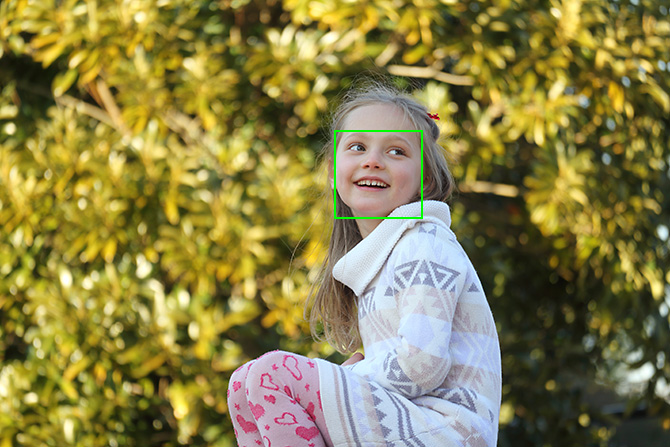
\includegraphics[height=4.0cm]{../src/output/face_box.png}
    }
    \subfigure[保护人脸的同时缩小图像]{
        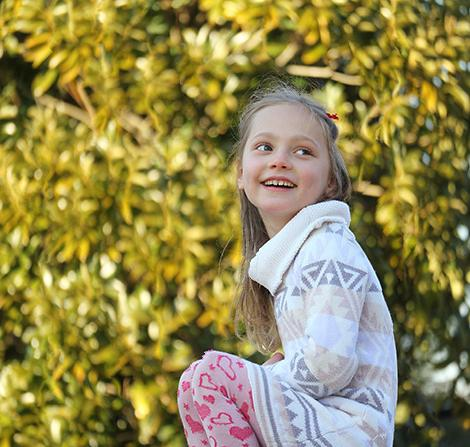
\includegraphics[height=4.0cm]{../src/output/face_protect.jpg}
    }
    \caption{受保护的人脸}
    \label{fig:face_protect}
\end{figure}

\section{优化细缝顺序}

在基础的Seam Carving算法中,如果需要同时改变图像的宽和高,并使得删除细缝的总能量最小,我们可以利用动态规划决定水平和竖直细缝删除的顺序。

具体来说,给定大小为$n\times m$的图像,需要放缩到$n'\times m'$,构造矩阵$T$,其中$T(r,c)$表示图像放缩到$(n-r)\times (m-c)$,得到下列状态转移方程。
\begin{equation}
    \begin{split}
        T(r,c) = \min(&T(r-1,c)+E(s^x(I_{n-r-1\times m-c})),\\
        &T(r,c-1)+E(s^y(I_{n-r\times m-c-1})))
    \end{split}
\end{equation}

其中$E(s^x)$表示竖直细缝的最小能量,$E(s^y)$表示水平细缝的最小能量。

我们将原图的宽高均缩小50像素,$T$矩阵及回溯路径和最终结果如\Cref{fig:opt_seam_order}。

\begin{figure}[H]
    \centering
    \subfigure[原图]{
        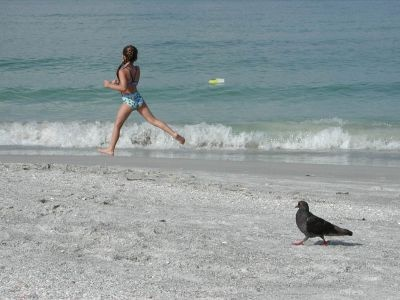
\includegraphics[width=0.4\textwidth]{../src/fig/beach.jpg}
    }
    \subfigure[$T$矩阵及回溯路径]{
        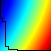
\includegraphics[width=0.2\textwidth]{../src/output/beach_opt_path.jpg}
    }
    \subfigure[最优缩小结果]{
        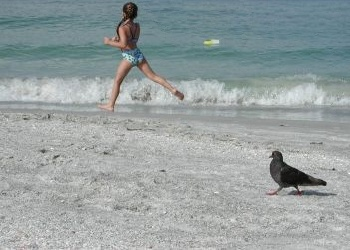
\includegraphics[width=0.3\textwidth]{../src/output/beach_opt_down.jpg}
    }
    \caption{最优细缝顺序}
    \label{fig:opt_seam_order}
\end{figure}

\section{更多工作}

我将Seam Carving算法进行了封装,发布了一个Python包到PyPI:\url{https://pypi.org/project/seam-carving/},可通过pip安装使用。代码已发布在GitHub:\url{https://github.com/li-plus/seam-carving},欢迎Star。

\bibliographystyle{plain}
\bibliography{report}

\end{document}
